\documentclass[conference]{IEEEtran}
\usepackage{graphicx}
\usepackage{cite}
\usepackage{listings}
\usepackage{xcolor}
\usepackage{tikz}
\usetikzlibrary{shapes, arrows, positioning}
\usepackage{caption}
\usepackage{graphicx}
\documentclass{article}
\usepackage[utf8]{inputenc}
\usepackage[backend=biber]{biblatex}

\addbibresource{bibliography.bib}

\lstdefinelanguage{VDM++}{
  morekeywords={types, public, private, instance, variables, inv, operations, return, class, seq, of, nat1, nat, real, bool, map, set, elems, let, if, then, end},
  sensitive=true,
  morecomment=[l]{--},       % Comentarios de una línea
  morestring=[b]",           % Definición de cadenas de texto
  basicstyle=\ttfamily,
  keywordstyle=\color{blue}\bfseries,
  commentstyle=\color{gray}\itshape,
  stringstyle=\color{green}\bfseries,
}

\lstset{
  language=VDM++,           % Usar el lenguaje VDM++ definido
  numbers=none,             % Desactivar la numeración de líneas
  basicstyle=\ttfamily\small, % Estilo de letra
  breaklines=true,          % Dividir líneas largas automáticamente
  frame=single,             % Marco alrededor del código
  rulecolor=\color{black},  % Color del marco
}


\title{Especificación Formal y Validación de un Sistema de Detección de Metales Pesados en el Agua}
\author{
    \IEEEauthorblockN{
        M. Pinazo\IEEEauthorrefmark{$1$}, 
        A. Vasquez\IEEEauthorrefmark{$2$}, 
        J. Ramos\IEEEauthorrefmark{$3$}, 
        J. Quispe\IEEEauthorrefmark{$4$}, 
        F. Perez\IEEEauthorrefmark{$5$},
        M. Molina\IEEEauthorrefmark{$6$}
    }
    \IEEEauthorblockA{Universidad La Salle de Arequipa, Perú}
    
    \IEEEauthorblockA{
        \IEEEauthorrefmark{$1$}mpinazov@ulasalle.edu.pe, 
        \IEEEauthorrefmark{$2$}avasquezl@ulasalle.edu.pe, 
        \IEEEauthorrefmark{$3$}jramoss@ulasalle.edu.pe,\\
        \IEEEauthorrefmark{$4$}jquispel@ulasalle.edu.pe,
        \IEEEauthorrefmark{$5$}fperezd@ulasalle.edu.pe
        \IEEEauthorrefmark{$6$}mmolinab@ulasalle.edu.pe
    }
}

\renewcommand\IEEEkeywordsname{Palabras clave}
\renewcommand\abstractname{Resumen}

\begin{document}
\maketitle

\begin{abstract}
El presente artículo establece una especificación formal y validación de un sistema de detección de metales pesados en el agua centrado en una solución de monitoreo automatizado y continuo. El sistema sugerido utiliza métodos electroquímicos para detectar la presencia de metales peligrosos como mercurio, arsénico y plomo. El sistema proporciona reportes detallados sobre la calidad del agua y alertas en tiempo real cuando las concentraciones de metales superan los niveles de seguridad. Para configurar el sistema, se utilizan métodos formales, particularmente VDM++, definiendo elementos importantes como estructuras de clases, tipos de datos y expresiones. Simulaciones y pruebas se realizan con muestras de agua limpia y contaminada para validar el sistema. Este método evita la necesidad de un monitoreo preciso a largo plazo de la calidad del agua y garantiza la precisión y confiabilidad del sistema.
\end{abstract}


\begin{IEEEkeywords}
    \textit{Metales pesados, Monitoreo de agua, VDM++, Validación, Especificación formal, Electroquímica, Alertas en tiempo real.}
\end{IEEEkeywords}

\section{Introducción}  
La contaminación del agua con metales pesados es un problema grave que afecta a muchas regiones del Perú, como Ayacucho, Junín, Piura, Puno, Moquegua y la provincia constitucional del Callao. La exposición a estos contaminantes, generados por actividades como la minería, la erosión natural, las prácticas agrícolas, el uso de fertilizantes, la mala gestión de residuos sólidos y los desechos industriales, pone en riesgo la salud y el medio ambiente.  

Metales pesados como el plomo, arsénico, mercurio y cadmio son altamente tóxicos y, al liberarse en cuerpos de agua, representan un peligro considerable para las comunidades que dependen de estos recursos hídricos. La exposición prolongada puede causar daños neurológicos, trastornos del sistema inmunológico, enfermedades renales, cáncer y afectar negativamente el desarrollo cognitivo en niños.  

A pesar de la gravedad del problema, los métodos de detección actuales suelen ser costosos, requieren equipos especializados y no permiten la detección en tiempo real, lo que incrementa el riesgo de incidentes de contaminación. En este contexto, surge la necesidad de un sistema automatizado, accesible y eficiente para la detección de metales pesados en el agua, capaz de operar en diversos contextos geográficos y económicos.  

Por ello, el presente trabajo tiene como objetivo general desarrollar un sistema basado en métodos formales para la detección automática y en tiempo real de metales pesados en el agua, contribuyendo así a la protección de la salud pública y el medio ambiente. Este sistema se enfocará en regiones vulnerables, donde el riesgo de exposición es elevado y la infraestructura actual es limitada.

\subsection{Objetivos Específicos}  
\begin{itemize}  
    \item Definir los parámetros y condiciones para el monitoreo continuo de metales pesados en el agua, como plomo, arsénico y mercurio.  
    \item Establecer los criterios para alertar a los usuarios cuando los niveles de metales pesados superen los límites permitidos.  
    \item Determinar el proceso de validación y calibración del sistema para garantizar su precisión a largo plazo.  
\end{itemize}  

\section{Trabajos Relacionados}

Los sistemas para detectar metales pesados en el agua pueden ser portátiles o no, lo que implica un alto consumo de recursos en algunos casos y un uso mínimo de recursos en otros, como se describe en los trabajos de Zhao y Li \cite{zhao2019}, quienes analizan las ventajas y limitaciones de los dispositivos portátiles para la detección de contaminantes. \\

La voltamperometría es un método que aplica un voltaje controlado a una muestra de agua a través de tres electrodos, según el artículo de Torres Llano \cite{torres2015}. Los átomos de mercurio de la muestra se depositan sobre el electrodo de trabajo a medida que aumenta el voltaje, generando una corriente eléctrica. Esta corriente cambia según la cantidad de mercurio presente, lo que permite calcular su concentración. Este proceso es extremadamente preciso y puede detectar concentraciones de mercurio muy bajas en el agua. Además, tecnologías recientes, como las basadas en nanotecnología, han mejorado la eficiencia de estos métodos, como se menciona en los trabajos de He y Yang \cite{he2020}. \\

Los autores Qi Ding, Chen Li, Haijun Wang, Chuanlai Xu y Hua Kuang \cite{ding2021} proponen el uso de técnicas electroquímicas recientes para detectar los iones de metales pesados presentes en el agua. Estos métodos permiten la detección de iones como Hg(II), Cd(II) y Pb(II) de manera rápida y efectiva. Además, se destacan por su facilidad de transporte y bajo costo. Por otro lado, Chen y Wang \cite{chen2018} presentan avances en sensores inteligentes que integran técnicas electroquímicas con sistemas portátiles, lo que mejora la sensibilidad y la versatilidad de los dispositivos de detección.

\subsection{Definici\u00f3n de Metales Pesados}

En la industria, los metales pesados desempe\u00f1an un papel esencial debido a sus propiedades físicas y químicas \u00fanicas, como la alta densidad y su resistencia a la corrosi\u00f3n. Estos metales son ampliamente utilizados en sectores como la manufactura, la electr\u00f3nica y la minería. Sin embargo, su liberaci\u00f3n al medio ambiente, a trav\u00e9s de efluentes industriales o pr\u00e1cticas inadecuadas de disposici\u00f3n de residuos, representa un desafío significativo para la salud p\u00fablica y la sostenibilidad ambiental \cite{sall2020, zaimee2021}.\\

La toxicidad de los metales pesados, incluso en concentraciones ínfimas, ha sido documentada ampliamente. Estos elementos tienden a acumularse en los organismos vivos, causando efectos adversos acumulativos a largo plazo. Por ejemplo, el plomo y el mercurio, que son altamente persistentes en el medio ambiente, pueden bioacumularse en la cadena alimentaria, afectando tanto a la fauna como a los seres humanos \cite{matthews2022, hughes2011}.\\

De los metales pesados analizados en este trabajo, se destacan los siguientes:

\begin{enumerate}
    \item \textbf{Plomo (Pb):} Su uso en baterías, pigmentos y soldaduras lo convierte en un metal crucial en la industria. Sin embargo, la exposici\u00f3n prolongada al plomo ha sido asociada con retrasos en el desarrollo cognitivo en ni\u00f1os y disfunci\u00f3n renal en adultos \cite{matthews2022, ding2021}.
    \item \textbf{Mercurio (Hg):} Ampliamente utilizado en la minería y en dispositivos como term\u00f3metros, el mercurio puede evaporarse f\u00e1cilmente, representando un riesgo tanto para los ecosistemas acu\u00e1ticos como para la salud humana \cite{sall2020, zhumanazar2022}.
    \item \textbf{Cadmio (Cd):} Este metal, presente en baterías recargables y pinturas, se clasifica como carcinog\u00e9nico. La exposici\u00f3n prolongada puede resultar en osteoporosis y disfunci\u00f3n renal severa \cite{rahimzadeh2017, park2022}.
    \item \textbf{Ars\u00e9nico (As):} En \u00e1reas donde el agua subterr\u00e1nea est\u00e1 contaminada con ars\u00e9nico, se han observado tasas elevadas de c\u00e1ncer de piel y disfunciones cardiovasculares \cite{hughes2011, truque2024}.
    \item \textbf{Cromo (Cr):} Aunque el cromo trivalente es esencial en trazas para el metabolismo humano, el cromo hexavalente es altamente t\u00f3xico, causando irritaciones severas y aumentando el riesgo de c\u00e1ncer pulmonar \cite{shin2023, park2022}.
\end{enumerate}

\subsection{Límites de Concentraci\u00f3n y Est\u00e1ndares para Metales Pesados en el Agua}

La presencia de metales pesados en fuentes de agua potable representa una preocupaci\u00f3n prioritaria para los organismos reguladores. La Organizaci\u00f3n Mundial de la Salud (OMS) y agencias como la Agencia de Protecci\u00f3n Ambiental (EPA) de los Estados Unidos han establecido límites de concentraci\u00f3n para proteger la salud humana. Por ejemplo, el límite recomendado para el plomo es de 0.01 mg/L, mientras que para el mercurio es de 0.006 mg/L \cite{truque2024, zaimee2021}.\\

El monitoreo continuo de estas concentraciones es fundamental, ya que la exposici\u00f3n prolongada puede derivar en problemas de salud irreversibles. Estudios recientes han destacado el papel de los sensores avanzados, que utilizan materiales como nanopartículas y polímeros conductores para mejorar la sensibilidad y la especificidad en la detecci\u00f3n de metales pesados \cite{yu2022, zhumanazar2022}. Estos avances tecnol\u00f3gicos han permitido la creaci\u00f3n de dispositivos port\u00e1tiles que combinan m\u00e9todos electroquímicos y \u00f3pticos para realizar mediciones en tiempo real \cite{ding2021, park2022}.\\

El dise\u00f1o del sistema propuesto incorpora estas tecnologías emergentes para ofrecer una soluci\u00f3n eficiente y econ\u00f3mica. Adem\u00e1s, los datos obtenidos se comparan con est\u00e1ndares internacionales, permitiendo emitir alertas cuando las concentraciones exceden los valores seguros establecidos \cite{rahimzadeh2017, shin2023}. Este enfoque no solo asegura la precisi\u00f3n del sistema, sino que tambi\u00e9n facilita su implementaci\u00f3n en contextos donde los recursos son limitados.\\

\subsection{Especificaci\u00f3n Formal para Sistemas de Detecci\u00f3n}

Para garantizar la confiabilidad y robustez del sistema, se ha empleado un enfoque de especificaci\u00f3n formal. Este m\u00e9todo permite describir de manera rigurosa los comportamientos esperados del sistema, minimizando posibles ambig\u00fcedades en su implementaci\u00f3n \cite{fitzgerald2007, woodcock1996}. Herramientas como Z y otros lenguajes de especificaci\u00f3n formal han demostrado ser eficaces en el dise\u00f1o y validaci\u00f3n de sistemas críticos, como los de detecci\u00f3n de contaminantes \cite{yu2022}.\\

Adem\u00e1s, la validaci\u00f3n del sistema se realiza a trav\u00e9s de pruebas exhaustivas que simulan condiciones reales de operaci\u00f3n. Estas pruebas incluyen escenarios de detecci\u00f3n de m\u00faltiples metales en concentraciones mixtas y la evaluaci\u00f3n de la respuesta del sistema frente a interferencias químicas \cite{rahimzadeh2017, ding2021}. Este enfoque asegura que el sistema cumpla con los requisitos establecidos, brindando resultados precisos y confiables en todo momento.\\

En resumen, el uso de tecnologías avanzadas combinado con m\u00e9todos formales de especificaci\u00f3n y validaci\u00f3n constituye un enfoque integral para abordar el problema de la detecci\u00f3n de metales pesados. Este enfoque no solo mejora la calidad de los datos obtenidos, sino que tambi\u00e9n refuerza la confianza en la toma de decisiones basada en evidencia científica.

\section{Especificaciones Formales y VDM++}
\subsection{VDM++}
La Vienna Development Method (VDM) es uno de los métodos formales más antiguos y establecidos orientados a modelos para el desarrollo de sistemas y software en entornos computacionales. Este método utiliza un conjunto de lenguajes rigurosamente fundamentados en la matemática para representar y analizar modelos de sistemas en las primeras fases del diseño. Esto permite evaluar las propiedades clave del sistema antes de realizar compromisos significativos relacionados con la implementación. Gracias a la construcción y análisis de estos modelos, es posible identificar áreas donde las especificaciones informales del sistema pueden ser incompletas o ambiguas, lo que proporciona una mayor confianza en que la implementación final respetará propiedades fundamentales, como la seguridad y la protección \cite{smith2021}.

\subsection{Definición de Clases}
En VDM++, las clases son bloques fundamentales que encapsulan tanto datos como operaciones. Las clases se definen mediante la especificación de sus atributos (variables de instancia) y métodos (funciones y operaciones). Cada clase también puede incluir invariantes que describen condiciones que deben mantenerse verdaderas a lo largo de la vida de la clase \cite{fitzgerald2009}.

\begin{figure}[h]
    \centering
    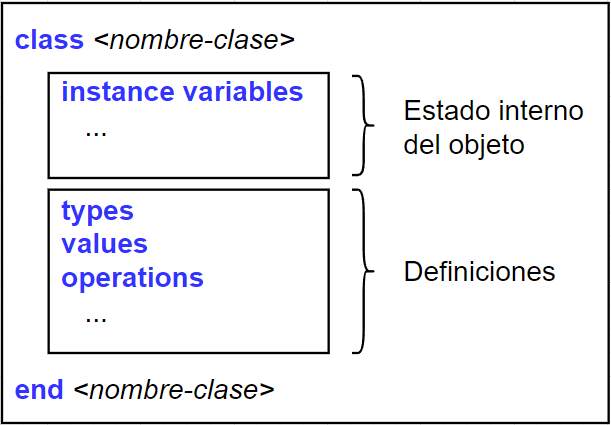
\includegraphics[width=0.5\textwidth]{Recursos/estructura_clases_vdm.png}
    \caption{Estructura básica de formalización de clases en VDM++}
\end{figure}

\subsection{Tipos}
VDM++ soporta una amplia variedad de tipos, tanto básicos como estructurados. Entre los tipos básicos se incluyen enteros, reales, booleans, y caracteres, mientras que los tipos estructurados pueden ser secuencias, conjuntos, y tuplas. Además, los tipos definidos por el usuario permiten una mayor flexibilidad y robustez en la modelización de sistemas complejos \cite{woodcock1996}.

\begin{figure}[h]
    \centering
    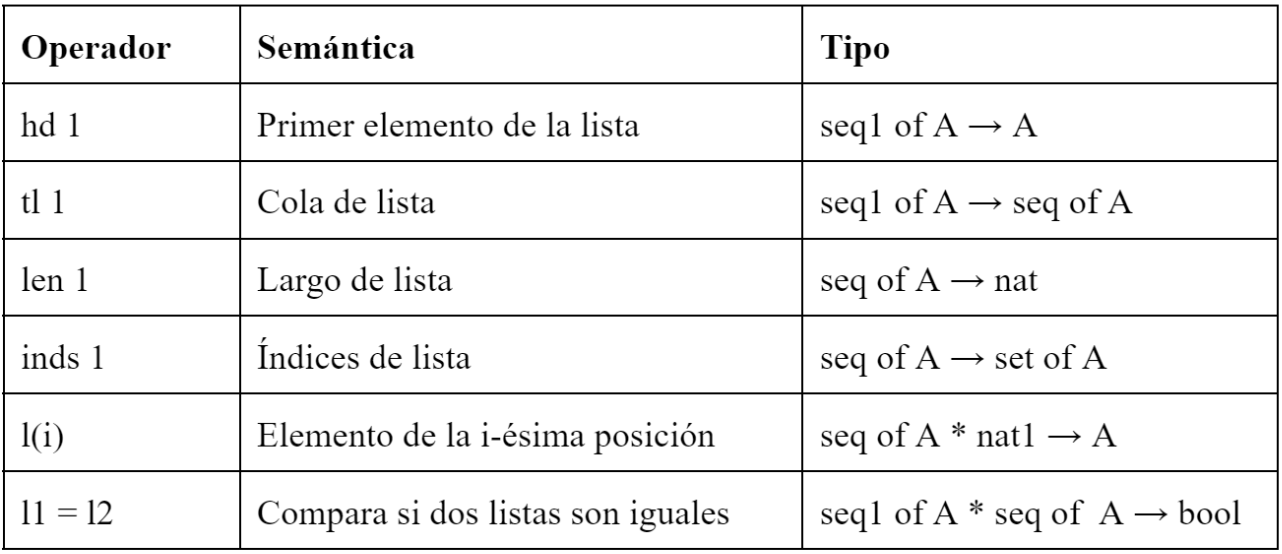
\includegraphics[width=0.5\textwidth]{Recursos/tipos_variables_vdmpp.png}
    \caption{Operaciones Formales de tipo secuencia en VDM++}
\end{figure}

\subsection{Expresiones}
Las expresiones en VDM++ están definidas de manera formal utilizando operadores matemáticos y lógicos. Estas expresiones pueden ser aritméticas, booleanas o relacionales, y se emplean para definir propiedades del sistema, como las precondiciones y postcondiciones de funciones y operaciones, así como las invariantes de las clases \cite{fitzgerald2009}.




\section{Propuesta}
\subsection{Requerimientos Funcionales del Sistema}
Para la determinación de los requerimientos en el sistema de detección de metales pesados en el agua, se debe de tener en cuenta los siguientes:

\begin{itemize}
    \item R1. Detección Automatizada: El sistema debe ser capaz de detectar automáticamente la presencia de metales pesados específicos en muestras de agua.
    \item R2. Alerta en Tiempo Real: Debe generar alertas en tiempo real cuando los niveles de metales pesados superen los límites de seguridad establecidos.
    \item R3. Monitoreo Continuo: El sistema debe poder realizar un monitoreo continuo de la calidad del agua en ubicaciones específicas.
    \item R4. Generación de Reportes: Debe poder generar reportes detallados sobre los niveles de contaminación, incluyendo gráficos y análisis históricos.
    \item R5. Calibración y Mantenimiento: El sistema debe incluir funcionalidades para la calibración y el mantenimiento regular de los sensores de detección.
\end{itemize}

\subsection{Diagrama de Clases}
El diagrama de clases se mostrará a continuación.

\begin{figure}[h]
    \centering
    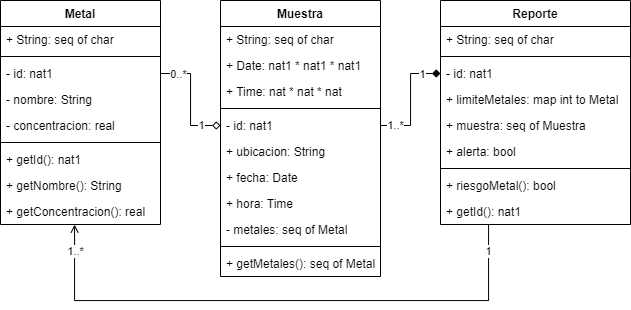
\includegraphics[width=0.5\textwidth]{Recursos/Metodos_Formales-DCL.png}
    \caption{Diagrama de Clases para la Especificación Formal y Validación de un Sistema de Detección de Metales Pesados en el Agua.}
\end{figure}

\newpage

\subsection{Sistema de Control}
El sistema de detección de metales pesados en el agua se formaliza a través de tres entidades principales: \texttt{Metal}, \texttt{Muestra}, y \texttt{Reporte}. A continuación, se describe cada uno de estos elementos.

La clase \texttt{Metal} representa cada tipo de metal presente en las muestras de agua. Los atributos de la clase son:
\begin{itemize}
    \item \textbf{id\_metal}: Identificador único para cada tipo de metal.
    \item \textbf{nombre}: Nombre descriptivo del metal (por ejemplo, mercurio o plomo) [1].
    \item \textbf{concentracion}: Concentración del metal en la muestra, expresada en unidades de partes por millón (ppm) [2], [3].
\end{itemize}

La clase \texttt{Muestra} captura la información de cada recolección de datos en el sistema:
\begin{itemize}
    \item \textbf{id\_muestra}: Identificador de la muestra.
    \item \textbf{ubicacion}: Descripción de la ubicación donde se toma la muestra.
    \item \textbf{fecha}: Fecha de recolección de la muestra.
    \item \textbf{tiempo}: Hora exacta de la recolección.
    \item \textbf{metales}: Lista de metales presentes en la muestra con sus respectivas concentraciones [4], [5].
\end{itemize}

La clase \texttt{Reporte} sintetiza los datos obtenidos de varias muestras y permite identificar riesgos:
\begin{itemize}
    \item \textbf{id\_reporte}: Identificador único del reporte generado.
    \item \textbf{limiteMetales}: Mapa que asocia el nombre del metal con su concentración límite aceptable [6].
    \item \textbf{muestra}: Lista de muestras que forman parte del reporte.
    \item \textbf{alerta}: Indica si hay alerta por sobrepasar los límites de concentración de metales [7].
\end{itemize}

El sistema emitirá una alarma en caso de que las concentraciones de los metales detectados superen los valores permitidos. La función \texttt{alertaRiesgo()} calculará si la concentración de algún metal es peligrosa para la salud humana, generando una señal de alerta [8].

\section{Especificación Formal}

\subsection{Clase Metal}

La clase \textbf{Metal} representa un metal detectado en una muestra de agua. Los atributos principales son:

\begin{itemize}
    \item \texttt{id}: Un identificador único para el metal.
    \item \texttt{nombre}: El nombre del metal, representado como una secuencia de caracteres.
    \item \texttt{concentracion}: La concentración del metal en la muestra, que debe ser un número real positivo.
\end{itemize}

Además, la clase contiene dos invariantes:

\begin{itemize}
    \item La longitud del nombre debe ser mayor que cero.
    \item La concentración debe ser mayor que cero.
\end{itemize}

El código en VDM++ de la clase es el siguiente:

\begin{lstlisting}
class Metal

types
public String = seq of char

instance variables
private id: nat1;
private nombre: String;
private concentracion: real;

inv len nombre > 0;
inv concentracion > 0;

operations
public Metal: nat1 * String * real ==> Metal
Metal(i, nom, con) == ( id := i; nombre := nom;
	concentracion := con; );

public getId: () ==> nat1
getId() == ( return id; );

public getConcentracion: () ==> real
getConcentracion() == ( return concentracion; );

end Metal
\end{lstlisting}

\subsection{Clase Muestra}

La clase \textbf{Muestra} modela una muestra de agua que contiene diferentes metales. Los atributos principales de esta clase son:

\begin{itemize}
    \item \texttt{id}: Un identificador único de la muestra.
    \item \texttt{ubicacion}: La ubicación donde se tomó la muestra.
    \item \texttt{fecha} y \texttt{hora}: La fecha y la hora en que se tomó la muestra.
    \item \texttt{metales}: Una secuencia de metales que se detectaron en la muestra.
\end{itemize}

Los invariantes de la clase aseguran que:

\begin{itemize}
    \item La ubicación no sea vacía.
    \item La secuencia de metales contenga al menos un metal.
\end{itemize}

El código en VDM++ de la clase es el siguiente:

\begin{lstlisting}
class Muestra
types
public String = seq of char;
public Date = nat1 * nat1 * nat1;
public Time = nat * nat * nat;

instance variables
private id: nat1;
public ubicacion: String;
public fecha: Date;
public hora: Time;
private metales: seq of Metal;

inv len ubicacion > 0;
inv len metales > 0;

operations
public Muestra: nat1 * String * Date * Time * seq of Metal ==> Muestra
Muestra(i, ubi, fec, hor, metal) == ( id := i; ubicacion := ubi;
	fecha := fec; hora := hor; metales := metal;
);

public getMetales: () ==> seq of Metal
getMetales() == ( return metales; );

end Muestra
\end{lstlisting}

\subsection{Clase Reporte}

La clase \textbf{Reporte} almacena la información sobre múltiples muestras y define los límites permitidos para las concentraciones de metales. Los atributos principales son:

\begin{itemize}
    \item \texttt{id}: Un identificador único para el reporte.
    \item \texttt{limiteMetales}: Un mapa que relaciona los identificadores de los metales con los límites de concentración permitidos.
    \item \texttt{muestras}: Una secuencia de muestras que se han tomado.
    \item \texttt{alerta}: Un valor booleano que indica si se ha detectado un riesgo.
\end{itemize}

Los invariantes de la clase aseguran que:

\begin{itemize}
    \item La secuencia de muestras no sea vacía.
    \item El mapa de límites de metales contenga al menos un valor.
\end{itemize}

La operación \texttt{riesgoMetal} evalúa cada muestra y verifica si la concentración de algún metal excede los límites permitidos. Si esto ocurre, se activa la alerta.

El código en VDM++ de la clase es el siguiente:

\begin{lstlisting}
class Reporte
types
public String = seq of char;

instance variables
private id: nat1;
public limiteMetales: map int to Metal;
public muestras: seq of Muestra;
public alerta: bool;

inv len muestras > 0;
inv card limiteMetales > 0;

operations
public Reporte: nat1 * map int to Metal * seq of Muestra * bool ==> Reporte
Reporte(i, lim, ms, alert) == ( id := i; limiteMetales := lim;
  muestras := ms; alerta := alert; );

public riesgoMetal: () ==> bool
riesgoMetal() == (
  for all m in set elems muestras do (
    let metales = m.getMetales() in (
      for all metal in set elems metales do (
        let limite = limiteMetales(metal.getId()) in (
          if metal.getConcentracion() > limite.getConcentracion() then
            return true;
        )
      )
    )
  );
  return false;
);

end Reporte
\end{lstlisting}

\section{Validación}
Para la realización de la validación se implementó la clase Analisis, donde se crearon los objetos necesarios de los tipos Metal, Muestra, Reporte. Además, se implementó los métodos para su creación y adecuado funcionamiento.

\begin{lstlisting}
class Analisis

types
public String = seq of char;

instance variables
private metales: seq of Metal;
private muestras: seq of Muestra;
private reportes: seq of Reporte;
private limites: map int to Metal;
private peligro: seq of String;

operations
public Analisis: () ==> Analisis
Analisis() == ();

public valoresPrueba1: () ==> () 
valoresPrueba1() == (
	limites := {1 |-> new Metal(1, "Plomo", 10.0), 2 |-> new Metal(2, "Mercurio", 6.0), 3 |-> new Metal(3, "Arsénico", 4.0)};
	metales := [new Metal(1, "Plomo", 12.5), new Metal(2, "Mercurio", 5.0), new Metal(3, "Arsénico", 3.2)];
	muestras := [new Muestra(1, "Laboratorio A", mk_(2024, 10, 20), mk_(14, 30, 0), [metales(1), metales(2)]), new Muestra(2, "Laboratorio B", mk_(2024, 10, 21), mk_(16, 0, 0), [metales(2), metales(3)])];
	reportes := [new Reporte(1, limites, muestras, false), new Reporte(2, limites, muestras, false)];
);

public valoresPrueba2: () ==> () 
valoresPrueba2() == (
	limites := {1 |-> new Metal(1, "Plomo", 10.0), 2 |-> new Metal(2, "Mercurio", 6.0),  3 |-> new Metal(3, "Arsenico", 4.0)};
	metales := [new Metal(1, "Plomo", 4.5), new Metal(2, "Mercurio", 5.0), new Metal(3, "Arsenico", 3.2)];
	muestras := [new Muestra(1, "Laboratorio A", mk_(2024, 09, 20), mk_(14, 30, 0), [metales(1), metales(2)]), new Muestra(2, "Laboratorio B", mk_(2024, 10, 21), mk_(16, 0, 0), [metales(2), metales(3)])];
	reportes := [new Reporte(1, limites, muestras, false), new Reporte(2, limites, muestras, false)];
);

public ejecutarAnalisis: () ==> String
ejecutarAnalisis() == (
  for all reporte in set elems reportes do (
    if reporte.riesgoMetal() then
		return "PELIGRO! CONCENTRACION DANINA";
  );
  return "SITUACION SEGURA";
);

end Analisis
\end{lstlisting}


A continuación, se presenta el uso de la clase Analisis, para la ejecución de las pruebas establecidas de funcionamiento del Sistema de Detección.
\begin{figure}[h]
    \centering
    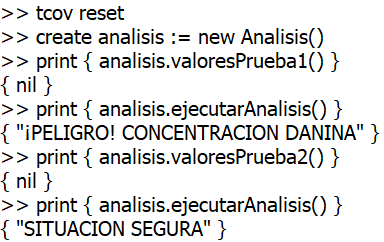
\includegraphics[width=0.5\textwidth]{Recursos/RealizandoPruebas.png}
    \caption{Realizando Pruebas con la clase Analisis.}
\end{figure}


Por consiguiente, se presenta la construcción del Coverage de las clases de nuestro Sistema de Detección, la cual consta de un 100\%. Para ello, se muestra la primera parte de los resultados del Coverage.
\begin{figure}[h]
    \centering
    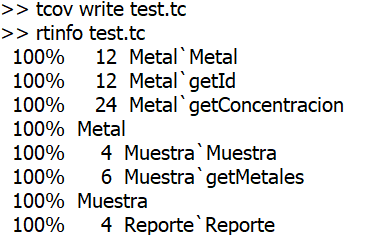
\includegraphics[width=0.5\textwidth]{Recursos/AnalisisCoverage1.png}
    \caption{Realizando Analisis de Coverage, Parte 1.}
\end{figure}

Finalmente, se muestra la segunda parte de los resultados del Coverage del Sistema de Detección.

\begin{figure}[h]
    \centering
    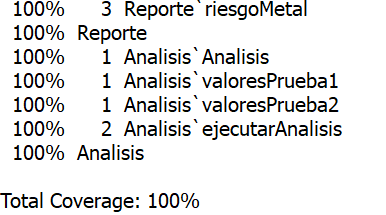
\includegraphics[width=0.5\textwidth]{Recursos/AnalisisCoverage2.png}
    \caption{Realizando Analisis de Coverage, Parte 1.}
\end{figure}
\section{Model Checking}
Para nuestro sistema de detección de metales pesados, se define un modelo que involucra dos subsistemas independientes que aseguran no estar simultáneamente en estado de alerta.

\subsection*{Variables del Modelo}
\begin{itemize}
    \item \textbf{System1:} Puede estar en los estados \textit{AlertaOn} o \textit{AlertaOff}.
    \item \textbf{System2:} Puede estar en los estados \textit{AlertaOn} o \textit{AlertaOff}.
\end{itemize}

\subsection*{Transiciones del Modelo}
Las transiciones para cada subsistema son las siguientes:
\begin{itemize}
    \item \textbf{System1:}
    \begin{itemize}
        \item Desde \textit{AlertaOff}, puede ir a \textit{AlertaOn} o permanecer en \textit{AlertaOff}.
        \item Desde \textit{AlertaOn}, solo puede ir a \textit{AlertaOff}.
    \end{itemize}
    \item \textbf{System2:}
    \begin{itemize}
        \item Desde \textit{AlertaOff}, puede ir a \textit{AlertaOn} o permanecer en \textit{AlertaOff}.
        \item Desde \textit{AlertaOn}, solo puede ir a \textit{AlertaOff}.
    \end{itemize}
\end{itemize}

\subsection*{Especificaciones del Modelo}
Las siguientes especificaciones aseguran el comportamiento correcto de los subsistemas:
\begin{itemize}
    \item \textbf{CTL:}
    \begin{itemize}
        \item $AG \neg(System1 = AlertaOn \land System2 = AlertaOn)$: Siempre es cierto que ambos sistemas no están en estado \textit{AlertaOn} simultáneamente.
        \item $EF\ System1 = AlertaOn$: Eventualmente, el sistema 1 llega al estado \textit{AlertaOn}.
        \item $EF\ System2 = AlertaOn$: Eventualmente, el sistema 2 llega al estado \textit{AlertaOn}.
        \item $AG\ (System1 = AlertaOff \rightarrow AX\ System1 = AlertaOn)$: Si \textit{System1} está en \textit{AlertaOff}, en el siguiente estado puede ir a \textit{AlertaOn}.
    \end{itemize}
    \item \textbf{LTL:}
    \begin{itemize}
        \item $F\ (System1 = AlertaOn)$: En algún momento, \textit{System1} estará en \textit{AlertaOn}.
        \item $G\ (System1 = AlertaOn \rightarrow X\ System1 = AlertaOff)$: Siempre que \textit{System1} esté en \textit{AlertaOn}, cambiará a \textit{AlertaOff} en el siguiente estado.
    \end{itemize}
\end{itemize}

\subsection*{Descripción del Modelo}
El modelo simula dos sistemas que operan independientemente con transiciones entre estados \textit{AlertaOn} y \textit{AlertaOff}. Garantiza que ambos sistemas no estén en estado de alerta simultáneamente.

\begin{lstlisting}
MODULE main
VAR
  System1 : {AlertaOn, AlertaOff};
  System2 : {AlertaOn, AlertaOff};

ASSIGN
  init(System1) := AlertaOff;
  init(System2) := AlertaOff;

  next(System1) := case
    System1 = AlertaOff : {AlertaOn, AlertaOff};
    System1 = AlertaOn : {AlertaOff};
    TRUE : System1;
  esac;

  next(System2) := case
    System2 = AlertaOff : {AlertaOn, AlertaOff};
    System2 = AlertaOn : {AlertaOff};
    TRUE : System2;
  esac;

SPEC AG !(System1 = AlertaOn & System2 = AlertaOn);
SPEC EF System1 = AlertaOn;
SPEC EF System2 = AlertaOn;
SPEC AG (System1 = AlertaOff -> AX System1 = AlertaOn);

LTLSPEC F (System1 = AlertaOn);
LTLSPEC G (System1 = AlertaOn -> X System1 = AlertaOff);
\end{lstlisting}

A continuación se presenta nuestro contra ejemplo del modelo establecido en NuSMV.
\begin{lstlisting}
MODULE main
VAR
  System1 : {AlertaOn, AlertaOff};
  System2 : {AlertaOn, AlertaOff};

ASSIGN
  -- Inicializacion de los sistemas
  init(System1) := AlertaOff;
  init(System2) := AlertaOff;

  -- Transiciones para System1
  next(System1) := case
    System1 = AlertaOff : {AlertaOn, AlertaOff};
    System1 = AlertaOn : {AlertaOff};
    TRUE : System1;
  esac;

  -- Transiciones para System2
  next(System2) := case
    System2 = AlertaOff : {AlertaOn, AlertaOff};
    System2 = AlertaOn : {AlertaOff};
    TRUE : System2;
  esac;

-- Propiedad a verificar
SPEC AG !(System1 = AlertaOn & System2 = AlertaOn)

\end{lstlisting}
\section{Conclusión}
El sistema de detección de metales planteado es una herramienta fundamental para el monitoreo preciso y constante de contaminantes en entornos industriales, destacando especialmente en el contexto de la contaminación del agua en nuestro país, Perú. Este sistema proporciona un control confiable sobre las concentraciones de metales, facilitando la detección oportuna de riesgos vinculados a la presencia de metales pesados. Acelerando las intervenciones y minimizando los impactos negativos tanto en el medio ambiente como en las comunidades que dependen de fuentes de agua seguras. Esto es particularmente beneficioso, debido a la gran cantidad de actividades industriales como la minería que contribuyen significativamente a la contaminación de los recursos hídricos. En este sentido, el sistema no solo aporta la capacidad de respuesta ante concentraciones peligrosas, sino que también facilita la implementación de políticas de control y reducción de la contaminación, promoviendo así la protección de la salud pública y el medio ambiente.


% Incluye todas las referencias sin citarlas explícitamente en el texto
\nocite{*}
\printbibliography

\end{document}
